\documentclass[11pt]{article} % 11pt article, want AMS fonts.

\usepackage{amsmath,amsfonts,amssymb}
\usepackage{latexsym}
\usepackage{hyperref}
\usepackage{graphicx}
\graphicspath{ {./images/} }
\usepackage{setspace}
\usepackage{blindtext}
\usepackage[a4paper, total={6in, 8in}]{geometry}
\usepackage[demo]{graphicx}
\usepackage{subfig}
\usepackage{indentfirst}
\usepackage{changepage}
\usepackage{booktabs}

% \singlespacing
% \onehalfspacing
\spacing{1.15} %to change spacing if necessary 


\begin{document}

\title{How Much Is A Best Picture Oscar Worth?}
\author{Isabella Cha, Kevin Phung, Aryan Arora}
\date{June 1 2022}
\maketitle

\section{Introduction}
The Academy of Motion Picture Arts and Sciences granted the first Oscars in 1929, creating what is today the oldest, most visible, and most prestigious award in the film industry (Levy 2001). The Academy Awards, now officially the Oscars, has changed little since 1929 - the nominees and winners are still decided by the members of the Academy, the nominees are revealed a month or two before the awards ceremony, and the winners are announced at the ceremony.

The existing literature suggests that movies are “experience goods”, defined as “products which consumers choose, buy and use solely to experience and enjoy” (Sawhney and Eliashberg 1996). The intangible and experiential nature of movie consumption makes it difficult to judge movie quality before it is actually viewed; as such, consumers may seek other signals prior to the consumption experience (Bristor 1990; Harrison-Walker 2001; Y. Liu 2006). The Oscars, arguably the most important award in the movie industry, is thought to be an important signal in shaping consumer perceptions (Ginsburgh 2003). The movies that receive this honor go down in history as films of quality and prestige. As noted by Levy (2001), “No other award so well combines critical and popular judgment”. Through the Oscars, the Academy functions as peers, critics, and tastemakers — thus, the question of how much an Oscar is worth is a pertinent one. 

In this paper, we are particularly concerned with the ‘Best Picture’ award, the highest honor of the ceremony. We define “worth” as commercial success, as measured by box office revenues. We will use econometric tools to measure whether winning a Best Picture Oscar increases consumers’ demand for a movie by significantly increasing weekly box office revenues. Our results show that Best Picture nominations boost movies’ revenues, whereas the effect of a win is not significant.  



\section{Theoretical Framework}
A movie’s box office revenue is directly related to the number of consumers purchasing tickets to view the movie. Economic theory suggests that the number of tickets sold is a function of consumer demand for seeing a given movie. Factors affecting consumer’s demand are likely to include the number of theaters, theater run, budget, genre, rating, whether the movie features a “star”, and/or released around a holiday. 

\subsection{Determinants of Movie Demand} 
\setlength\parindent{0pt}

\begin{adjustwidth}{1cm}{}

\textbf{Number of theaters} \newline
More theaters implies that consumers have easier access to see a given movie; if a moviegoer is deciding between different movies, all else equal, then they are more likely to see the one screening closest to them. Some consumers may not decide what to watch until entering the theater, all else equal, the likelihood of watching a movie would increase with the movie being shown in more theaters. If no theaters were showing the movie, then ticket sales would effectively be zero. \\


\textbf{Budget}\newline
Higher budget could allow for more spending on factors that could improve movie quality, such as better camera equipment, higher quality editing, and better sound. In addition, a higher budget allows for more spending on advertising and promotion which would also increase demand. Previous studies suggest that high budget films generate more revenues (Deuchert et. al 2005), albeit with varying degrees of elasticity.  
\\

\textbf{Genre}\newline
 Film genres appeal differentially to moviegoers. For example, animated and family films are the most popular genre for children accompanied by parents, action/adventure films appeal to younger audiences, and dramas are more popular among older audiences (Redondd and Holbrook 2010). A movie’s strongest competition comes from other movies that are most alike in genre (Elberse 2005; Y. Liu 2006). From this, we postulate that movies in the same genre category may be substitutes; all else equal, a bigger number of substitutes would decrease quantity demanded. 
 \\

\textbf{MPAA Rating}\newline
The MPAA rating of movies may attract or repel certain audiences. G and PG rated movies may be more appealing to families, whereas R-rated movies may appeal to more mature audiences. However, the effect of MPAA ratings may be ambiguous: for instance, the presence of obscene language, explicit sex, and/or violence was reported as the second most important factor in avoiding R-rated movies (Moon et al. 2010) for R-rated movies. On the other hand, some studies suggest sexual content is intrinsically profitable precisely \textit{because} of its controversial nature (Pennington 2007). \\

\textbf{Holiday}\newline
Whether or not a movie was released around a holiday may be a determinant of movie demand. The number of moviegoers varies dramatically throughout the year according to Einav (2007), who observes a “seasonal pattern” of movie sales, with the biggest hits in the beginning of the Christmas holiday season. However, it is also plausible that consumers may prefer to stay at home with family rather than go to movie theaters on Christmas. \\

\textbf{Star Power}\newline
Star power is considered to be one of the key drivers of motion picture success, albeit with some controversy. As Bill Mechanic, former chairman of Twentieth Century Fox put it, “a guy stranded on an island without Tom Hanks is not a movie… there's no way to replace that kind of star power.”  Elberse (2007) finds that on the basis of a multiple regression model, star power has no significant box office sales. On the other hand, Prag and Casavant (1994) found that star power and winning an Academy Award are “unambiguous positive factors in a movie’s financial success.” 
\end{adjustwidth}


\setlength{\parindent}{20pt}

\section{Data}
\subsection{Data Collection} 
Our dataset includes all Oscar-Best picture nomianted movies that were released in the US after January 1, 2000, and which official domestic (US) running time did not exceed December 31, 2019. In order to isolate the effect of the Oscar event, we exclude films that were not nominated. We also decided to exclude movies running from 2020 and beyond due to the COVID-19 pandemic and the shutdown of theaters. We then collected data for our dependent variable and possible explanatory variables as outlined in our theoretical framework. 

Weekly box office returns, release dates, and budget information are taken from boxofficemojo.com. To check whether awards influence success, we look at weekly revenue (as opposed to gross revenues) to account for the income generated after the Oscars announcement, in order to be able to determine whether it is the Oscar announcement that triggered the additional income. It is also important to note that the industry operates on a weekly schedule --— much of the competition is over the weekend audience. Consequently, release dates are tabulated at the weekly level. 

Nominations, wins, details on genre, movie content ratings were taken from Internet Movie Database (IMDb). Additionally, data for movie budgets was scraped from The-Numbers (https://www.the-numbers.com/). Star power was constructed from Forbes, List of 100 Highest paid Actors and Actresses for each respective year. 

As final step, we merged and cleaned our datasets from various website using automated Python scripts. Our final dataset includes 125 movies and weekly revenue data for each movie. In total, we have 2999 observations. 

\subsection{Description of Variables}

\begin{table}[h]
\caption{Column names and definitions}
\resizebox{\textwidth}{!}{%
\begin{tabular}{cc}
\hline
\textbf{Variable Name} &
    \textbf{Definition} \\ \hline
    
\textit{WeeklyRevenue} &
  \begin{tabular}[c]{@{}l@{}}Revenues from US ticket sales, measured in USD. \\ Does not include DVD rentals, streaming purchases, or additional releases of the film.\end{tabular} \\ \hline
\textit{Week} &
  Current week in the calendar year. \\ \hline
\textit{Cumulative Weeks} &
  Number of weeks after release, starting from 1. \\ \hline
\textit{Weekly rank} &
  \begin{tabular}[c]{@{}l@{}} Rank of the movie relative to other movies in terms of revenue. \\ Gives us an idea of the movie’s performance relative to other \\ movies screening at the same week.\end{tabular} \\ \hline
\textit{Theaters} &
  \begin{tabular}[c]{@{}l@{}}Number of cinema cites showing the movie.\\ Only includes US theaters.\end{tabular} \\ \hline
\textit{Budget} &
  Movie production budget, measured in USD. \\ \hline
\textit{Genre (6 groupings)} &
  \begin{tabular}[c]{@{}l@{}}6 different genre groupings: \\ (1) Action, Adventure, Fantasy, Sci-Fi (AAFS); \\ (2) Drama,Comedy,Romance (DCR); \\ (3) Crime, Mystery, Horror, Thriller (CMHT); \\ (4) Biography, Sport, History, War (BSHW); \\ (5) Animation, musical, family (AMF); \\ (6) Western (W). \\ Each genre grouping is a dummy variable, which takes on a value of 1 \\ if the movie is classified as part of the grouping.\end{tabular} \\ \hline
\textit{Holiday (Constructed)} &
  \begin{tabular}[c]{@{}l@{}}A binary variable to indicate if a movie is released in the holiday season.\\ "Holiday season" is defined as the last 6 weeks of the calendar year.\end{tabular} \\ \hline
\textit{Star power (Constructed)} &
  \begin{tabular}[c]{@{}l@{}}A binary variable to indicate if the movie has star power. \\ A movie is classified as having star power if at least one of its \\ main cast members appears in Forbes list of 100 top-paid actors \\ and actresses in their respective year of release. \\ This classification is in similar fashion with previous studies \\ done on star power (Liu Y. 2006; Liu, A. et. al 2014).\end{tabular} \\ \hline
\textit{Oscar Nomination} &
  A binary variable if a movie was nominated for the Best Picture Oscar. \\ \hline
\textit{Oscar Win} &
  A binary variable if a movie won the Best Picture Oscar. \\ \hline
\end{tabular}}
\end{table}


\newpage


\section{Model Specification}

Given our economic theory for the variables we considered, we began by creating a model with all of our variables. We then ran F and T tests on the variables for which we did not have a strong enough economic theory and thus wanted to examine. We first ran an F test on both Genre and Ratings.

Our F test on Genre produced a statistically significant result at a 5\% significance level (p value = 0.0009393). This meant that the restriction (removing the genre dummy variables) significantly worsened the goodness of fit. 

Our F test on Rating did not produce a statistically significant result at a 5\% significance level (p value = 0.09054). This meant that the restriction (removing the rating dummy variables) did not significantly worsen the goodness of fit. 

Furthermore the T test on the star power explanatory variable did not provide a statistically significant result at a 1\% level of significance. Given that we did not have sufficient economic theory justifying star power as a predictor of film earnings, we held a high threshold to include it in the model (hence 1\%), and thus we decided to omit the variable. We also removed the interaction between cumulative gross earnings and and win for similar reasons (p value = 0.88290).

We then conducted tests for linearity and found non-linearity in our model which we resolved by logging the dependent variable: weekly earnings. This provided the following Histogram and QQ plot:

\begin{figure} [h]
    \centering
    \subfloat{{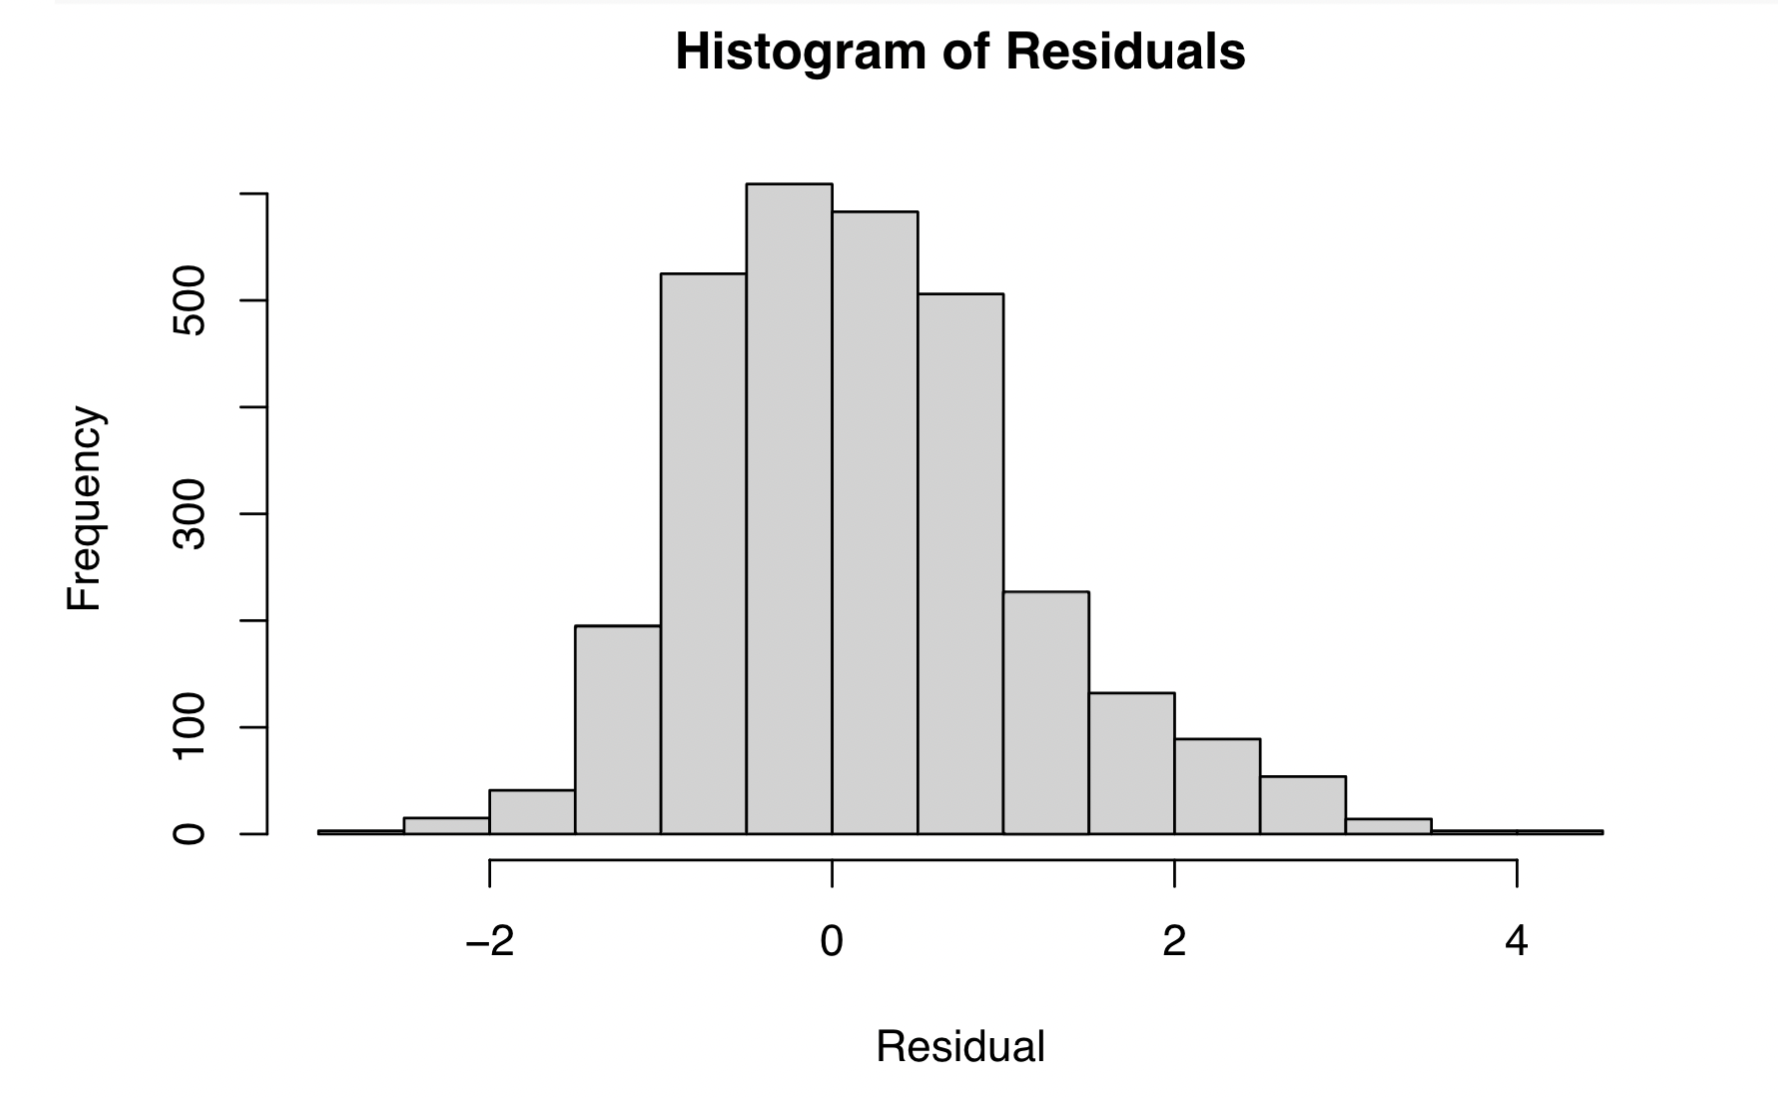
\includegraphics[scale = 0.22]{Histogram.png} }}%
    \qquad
    \subfloat{{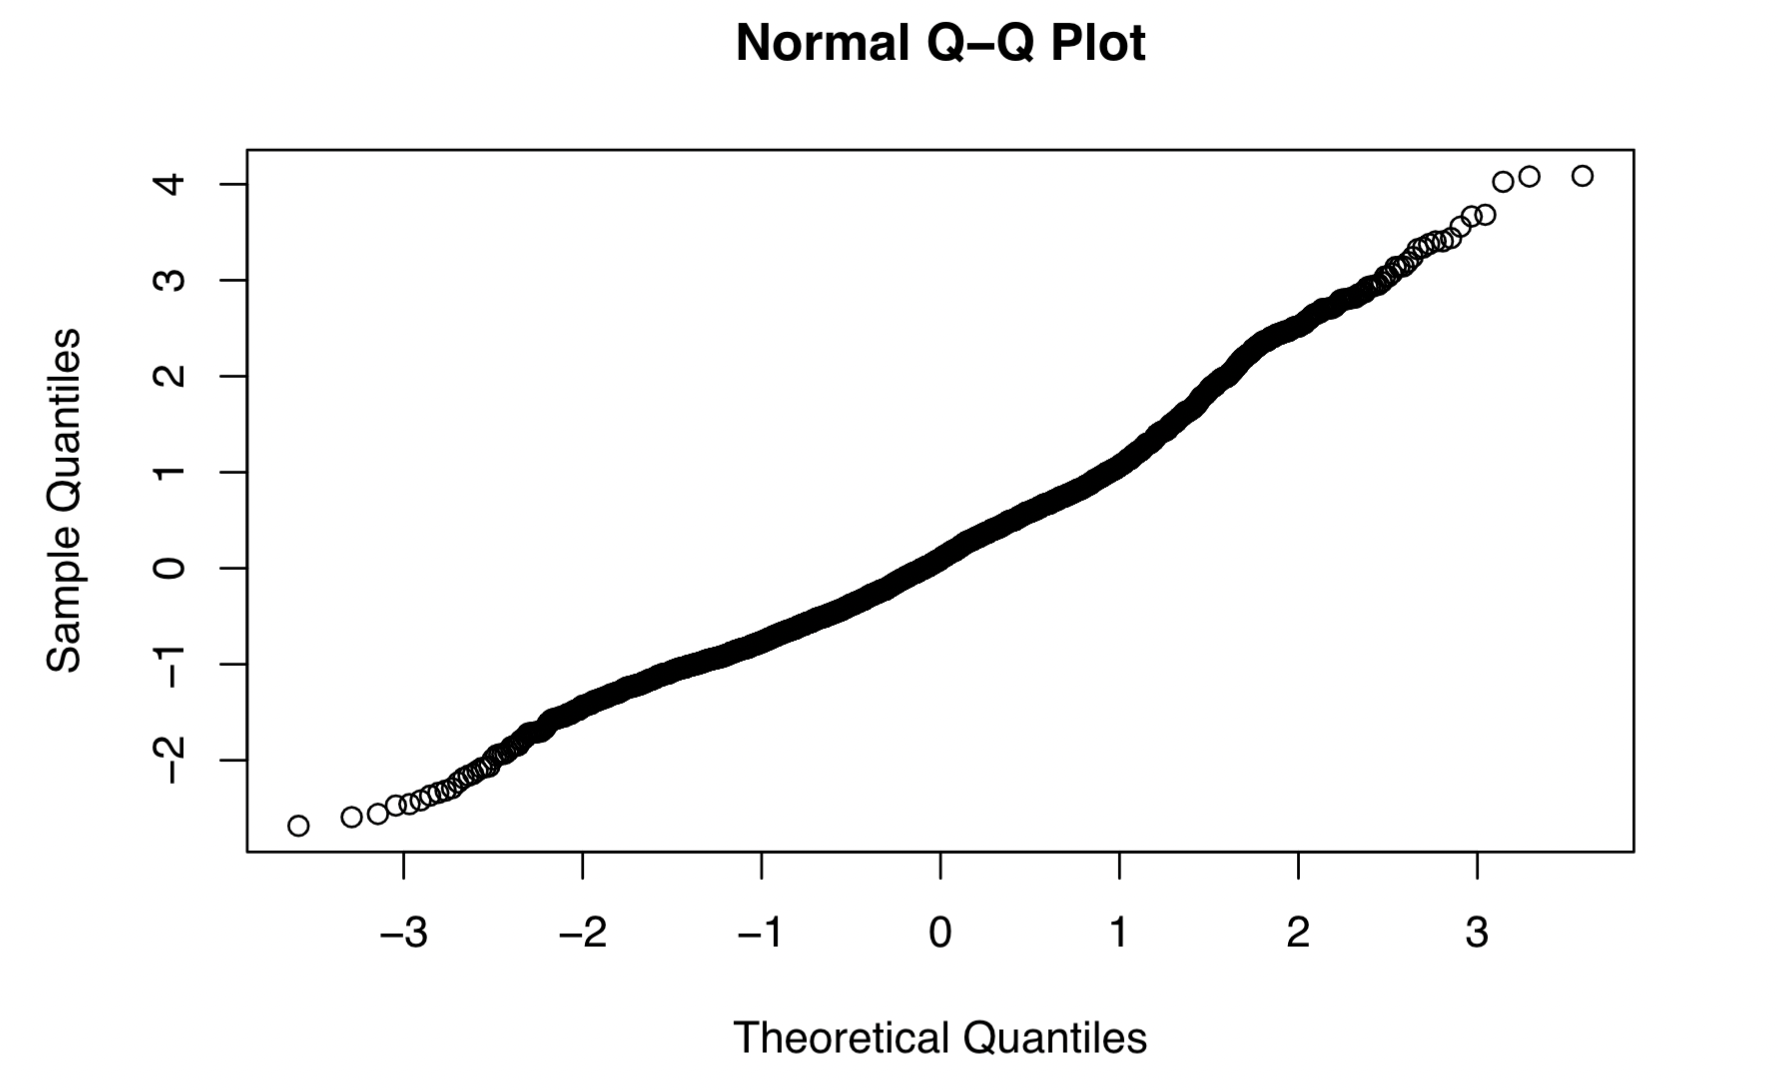
\includegraphics[scale = 0.22]{QQ Plot.png}}}%
    \label{fig:example}%
\end{figure}

We did not conduct a Shapiro-Wilk test, as the test is highly sensitive when we have a large sample size. At large sample sizes, the probability of rejecting the null hypothesis that the residuals are normally distributed becomes extremely large, leading to everything short of perfect normality being rejected by the test. 

Our Breusch-Pagan test for heteroskedascity produced a chi-square statistic that provided strong evidence of heteroskedasticity in our model. We then recalculated our standard errors using robust standard errors.


Finally we conducted a Durbin-Watson test for autocorrelation and and used a correlation matrix to evaluate multicollinearity. Given that our Durbin Watson statistic (1.685) fell within the range of 1.611 to 3.919(d=14 and no intercept), we did not see evidence of a concerning level of autcorrelation in our data. 

We found very little evidence of concerning multicollinearity. The 
weekly rating of the film and the cumulative weeks seemed to have strong multicollinearity. On a theoretical basis this makes sense—a film that maintains a significantly high weekly rating is likely to continue running for many cumulative weeks. What is important to clarify though is why we see a positive correlation between weekly rank and cumulative weeks. A successful movie that have been running for many weeks will start to have a lower rank (for instance a film that runs for 20 weeks may be the #1 movie for 8 weeks and then slip down to being #20 in weeks 8-12). Then it makes sense that a lower ranked movie, with a higher value for "weekly rank" (because 5 > 1 but being ranked #1 > #5) will be positively correlated with cumulative number of weeks.

A similarly high level of multicollinearity follows for the number of theaters and weekly rank. Here again, the theory suggests that this is to be expected—a highly ranked film will be in many theaters. We see a negative correlation here because a higher weekly rank (with a lower 'score' because 1 < 5 but being ranked #1 > #5) will mean you are likely in more theaters.  

Another case of multicollinearity was between cumulative number of weeks and nomination. We spoke about this briefly in our initial theory section but it made sense to us that a film that had been out for more cumulative weeks, and thus had the opportunity to be seen by a larger audience and more critics, would be more likely to be nominated (hence the positive correlation). This is why the films that are in contention for nomination are often strategically released during the holiday season. 

One final case of multicollinearity that did not come up as particularily noteworthy through our correlation matrix, but we believe is theoretically important to acknowledge, is the relationship between Nomination and a Best Picture Oscar Win. You cannot win if you are not nominated. In summary of these explanations, there exist some cases of multicollinearity in our data—but nothing concerning or unexplained by the economic theory underpinning our model.

\begin{center}
    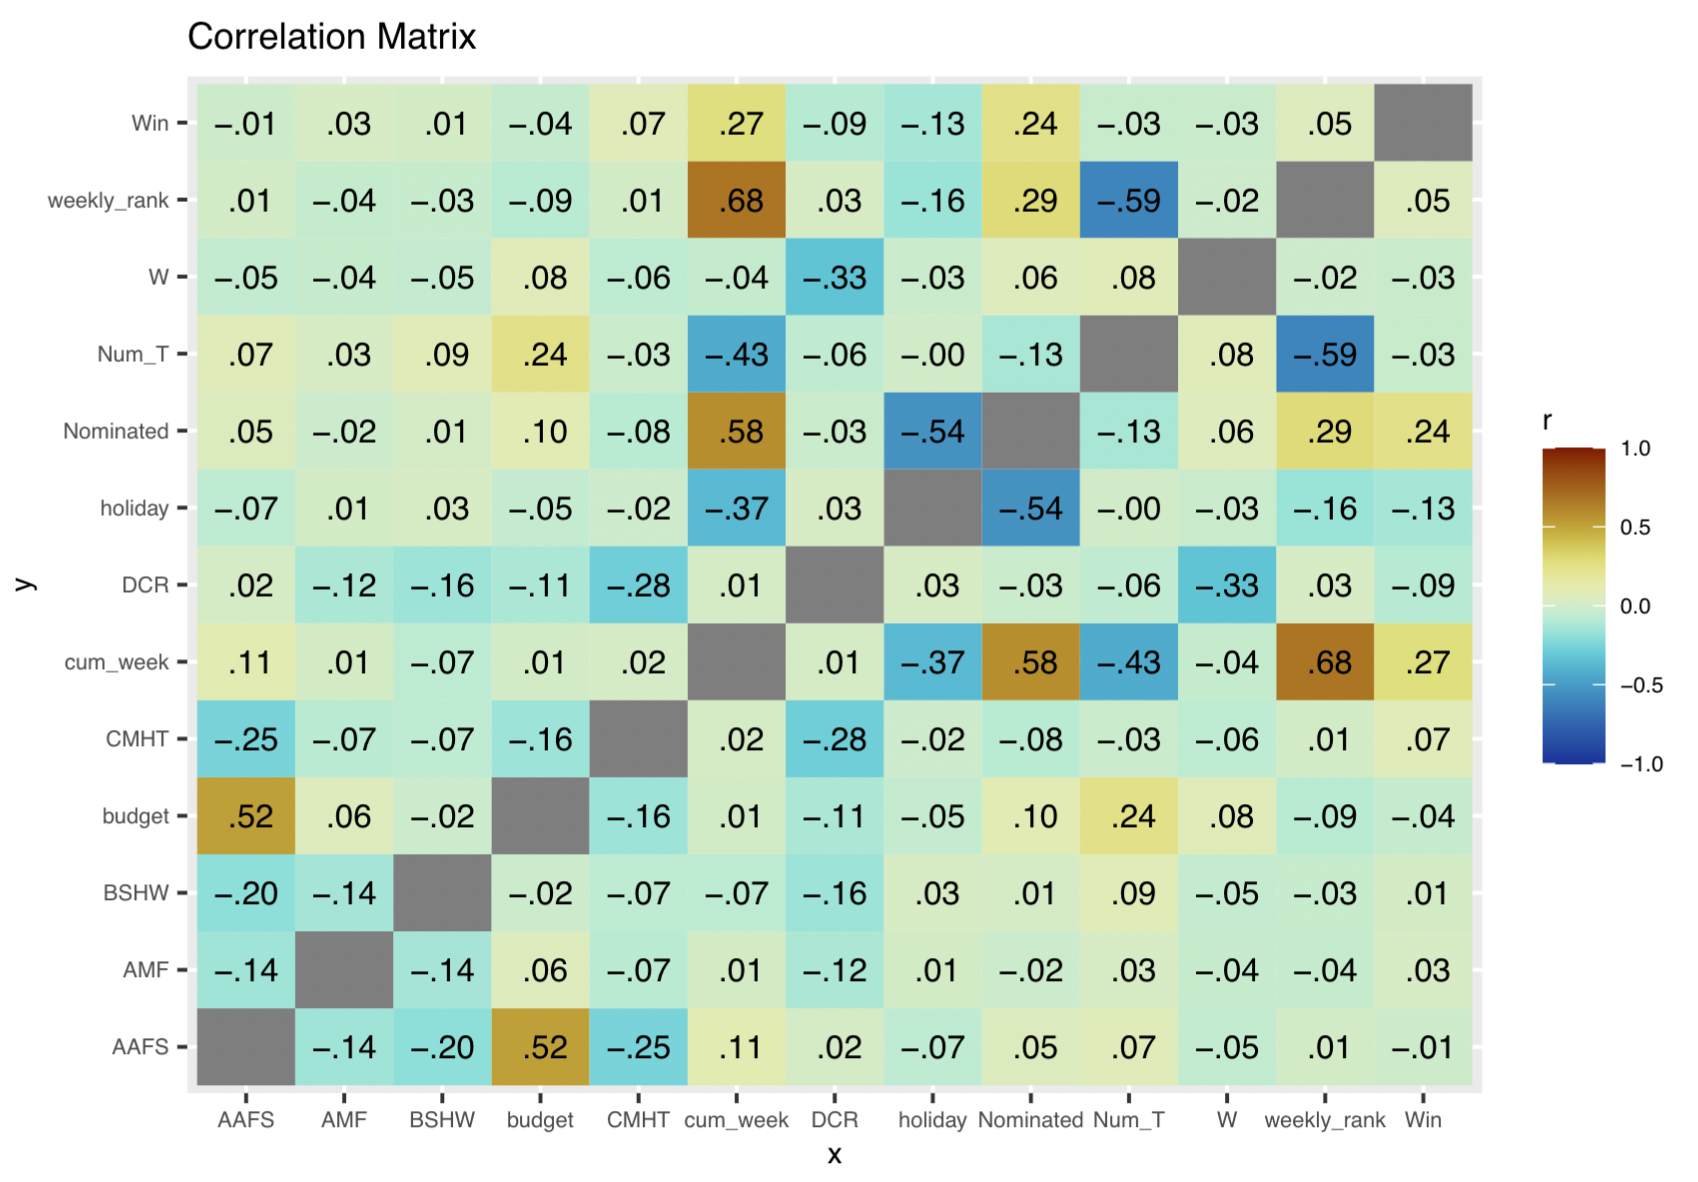
\includegraphics[scale = 0.5]{Correlation Matrix.png}
\end{center}

This produces our final model: 

\begin{center}
    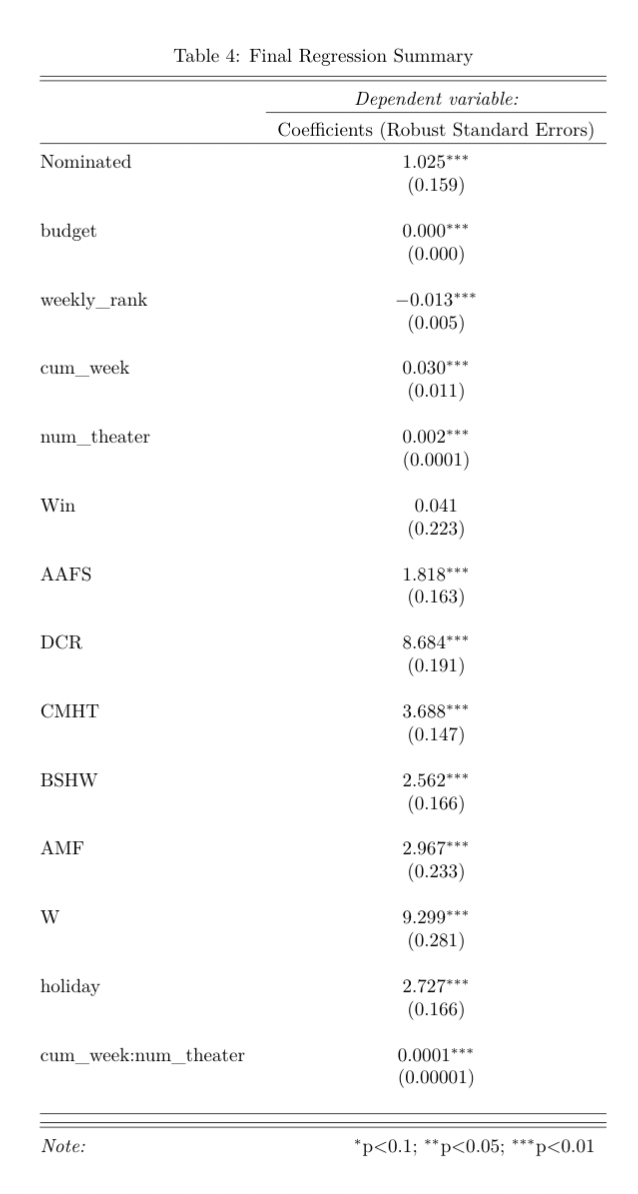
\includegraphics[scale = 1.0]{Regression Output.png}
\end{center}

\section{Empirical Results and Analysis}

Our goal is to estimate the degree to which the explanatory variables discussed in earlier sections are correlated with the weekly box-office revenues in our sample. To do so, we estimate a standard weekly revenue function of the form: 
$regression equation = \beta_0 + ... $
and the explanatory variables are defined as listed in Table #NUMBER. 

\subsection{Interpretation of Beta Coefficients}
We do not find evidence for the generated revenue in addition to nominations, since the coefficient for a Win is negative but not statistically significant. 

Based on our model results, holding everything else equal, \textit{Nomination} will lead to an increase in the median weekly revenue of a movie by a multiplicative factor of $e^{1.025}$ or $2.787$. Basically, median weekly revenue is \$2.787 higher if a movie has a nomination than without. 

Holding everything else equal, a 1 unit increase in \textit{Budget} will lead to an increase in the median weekly revenue of a movie by a multiplicative factor of $e9.808*10-9$ or $1.00000000981$.  Basically, median weekly revenue is \$1.00000000981 higher if a movie increases its budget by \$1.

Holding everything else equal, a 1 place decrease (from rank 1 to rank 2) in \textit{Weekly\_Rank} will lead to an decrease in the median weekly revenue of a movie by a multiplicative factor of $e^{-0.01302}$ or 0.98706439353.  Basically, median weekly revenue 1.294\% lower if  \textit{Weekly\_Rank} decreases by 1 spot.

Holding everything else equal, a 1 week increase in \textt{Cumulative\_Week}  will lead to an increase in the median weekly revenue of a movie by a multiplicative factor of $e^0.03036$ or 1.03082556437.  Basically, median weekly revenue is 3.083\% higher if \textit{Cumulative\_Week} increases by 1 week.

Holding everything else equal, an increase in the \textit{Number\_Of\_Theaters} the movie is shown in by 1 will lead to an increase in the median weekly revenue of a movie by a multiplicative factor of $e^{0.001721}$ or 1.00172248177.  Basically, median weekly revenue is 0.172\% higher if the number of theaters the movie is shown in  increases by 1 week.

Based on our model results, holding everything else equal, a $Win$ will lead to an increase in the median weekly revenue of a movie by a multiplicative factor of $e^{0.04079}$ or 1.04163333957. Basically, median weekly revenue is 4.163\%  higher if a movie has a win than without. Based on the p-value however, this result is not significant.

Based on our model results, holding everything else equal, a movie being shown during the $holiday$ will lead to an increase in the median weekly revenue of a movie by a multiplicative factor of $e^{2.727}$ or 15.287. Basically, median weekly revenue is 15.287 times higher if a movie is shown during the holidays than outside of it.

Based on our model results, holding everything else equal, an increase in the interaction between $cumulative\_week$ and $Number\_of\_Theatres$ by 1000 will lead to an increase in the median weekly revenue of a movie by a multiplicative factor of $e^{0.08877}$ or 15.287. Basically, median weekly revenue is 9.28\% higher if the interaction between $cumulative\_week$ and $Number\_of\_Theatres$ increases by 1000.

For the following interpretations, We will assume that the baseline Movie is one that only contains genres in the Action,Adventure,Fantasy,Sci-Fi (AAFS) categories. The numbers here may seem disproportionate at times, but that is due to the fact that many of these movies could be lumped under several categories at once. E.g.: Some movies are in both AAFS and DCR categories.


Based on our model results, holding everything else equal, a movie being only in the Drama,Comedy,Romance genres will lead to an increase in the median weekly revenue of a movie by a multiplicative factor of $\frac{e^{8.684}}{e^{1.818}}$ or 959.104. Basically, median weekly revenue is 959.1 times  higher if a movie has only Drama and/or Comedy and/or Romance as a genre when compared against a movie that only AAFS as genres.

Based on our model results, holding everything else equal, a movie being only in the Crime, Mystery, Horror, Thriller  genres will lead to an increase in the median weekly revenue of a movie by a multiplicative factor of $\frac{e^{3.688}}{e^{1.818}}$ or 6.49. Basically, median weekly revenue is 6.49 times  higher if a movie has only Crime and/or Mystery and/or Horror and/or Thriller as a genre when compared against a movie that only AAFS as genres.

Based on our model results, holding everything else equal, a movie being only in the Biography, Sport, History, War genres will lead to an increase in the median weekly revenue of a movie by a multiplicative factor of $\frac{e^{2.562}}{e^{1.818}}$ or 2.104. Basically, median weekly revenue is 2.104 times  higher if a movie has only Biography and/or Sport and/or History and/or War as a genre when compared against a movie that only AAFS as genres.

Based on our model results, holding everything else equal, a movie being only in the Animation, musical, family  genres will lead to an increase in the median weekly revenue of a movie by a multiplicative factor of $\frac{e^{2.967}}{e^{1.818}}$ or 3.155. Basically, median weekly revenue is 3.155 times  higher if a movie has only Animation and/or musical and/or family as a genre when compared against a movie that only AAFS as genres.

Based on our model results, holding everything else equal, a movie being only in the Western genre will lead to an increase in the median weekly revenue of a movie by a multiplicative factor of $\frac{e^{9.299}}{e^{1.818}}$ or 1774. Basically, median weekly revenue is 1774 times  higher if a movie has only Western as a genre when compared against a movie that only AAFS as genres. The reason this multiplier is so high is that we only have 2 movies under the 'Western' genre here(Gladiator and True Grit), and both pulled in huge amounts of money at the box office.

\subsection{Analysis}




\section{Limitations and Areas for Future Research}
Although our measure of a movie’s ‘success’ is weekly box office revenues, it is also important to acknowledge that the Academy does not blindly endorse the masses, given the Academy’s own proclamation that “excellence in filmmaking is the only factor [to] consider in casting votes” (National Academy, 2022). The votes are cast by, namely, members of the Academy who comprise of “gifted and skilled artists and craftsmen in the motion picture world” -- 8,100 members as of 2019). The panel of judges are chosen on an invite-only basis; the exact criterion is not known to the public. As such, commercial success and Oscar wins may only be associated to the extent that these supposed experts and moviegoers share the same taste. 

Moreover, the movie industry has undergone structural changes during the time frame 2000-2019 for which we collected our data. With the rise of Netflix and other streaming services, box office numbers measuring ticket sales are incomplete and don't show the full picture for the demand of a movie. Nowadays, consumers can enjoy a newly released movie in the comfort of their homes. For a more comprehensive analysis, we could look at user data from streaming services; however, this data is not publicly available and hence outside of the scope of our investigation. 

Our dataset also includes notable outliers such as \texit{Avatar}. For such blockbuster films, it is difficult to say whether awards influence success or whether the Academy goes with the flow or the Oscar win boosted revenues. Avatar, for example, made 140 millions USD in the first week alone. Due to complications in defining an exact threshold for excluding movies, however, we did not remove these observations — which may have biased our results. 

Further, we were working with time-series data but did not have the ability to use time series models, which limited the set of tools for model building to multi-variable regression analysis. 


\section{Conclusion}

\newpage
\section*{References}
\leftskip 0.3in
\parindent -0.3in

\noindent 

Deuchert,, E., Adjmah, K., & Pauly, F. (2005). For Oscar Glory or Oscar Money? Journal of Cultural Economics, 29(3), 159–176. http://www.jstor.org/stable/41810887 

Elberse, A. (2007). The Power of Stars: Do Star Actors Drive the Success of Movies? Journal of Marketing, 71(4), 102–120. http://www.jstor.org/stable/30164000 

Einav, L. (2007). Seasonality in the U.S. Motion Picture Industry. The RAND Journal of Economics, 38(1), 127–145. http://www.jstor.org/stable/25046296 
 
Ginsburgh, V. (2003). Awards, Success and Aesthetic Quality in the Arts. The Journal of Economic Perspectives, 17(2), 99–111. http://www.jstor.org/stable/3216859 

Levy E. (2001) Oscar Fever: The History and Politics of the Academy Awards (The Continuum International Publishing Group, New York). 

Liu, Y. (2006). Word of Mouth for Movies: Its Dynamics and Impact on Box Office Revenue. Journal of Marketing, 70(3), 74–89. http://www.jstor.org/stable/30162102

Liu, A., Liu, Y., & Mazumdar, T. (2014). Star power in the eye of the beholder: A study of the influence of stars in the movie industry. Marketing Letters, 25(4), 385–396. http://www.jstor.org/stable/24571121

Nelson, Randy & Donihue, Michael & Waldman, DM & Wheaton, C. (2001). What's an Oscar Worth? Economic Inquiry. 39. 1 - 6. 10.1111/j.1465-7295.2001.tb00046.x.

Redondo, Ignacio, and Morris B. Holbrook. “Modeling the Appeal of Movie Features to Demographic Segments of Theatrical Demand.” Journal of Cultural Economics 34, no. 4 (2010): 299–315. http://www.jstor.org/stable/41811062.
 
Rao, V. R., Ravid, S. A. (Avri), Gretz, R. T., Chen, J., & Basuroy, S. (2017). The impact of advertising content on movie revenues. Marketing Letters, 28(3), 341–355. http://www.jstor.org/stable/45214411

Moon, S., Bergey, P. K., & Iacobucci, D. (2010). Dynamic Effects among Movie Ratings, Movie Revenues, and Viewer Satisfaction. Journal of Marketing, 74(1), 108–121. http://www.jstor.org/stable/20619083 

Liu, Yong (2006), "Word of Mouth for Movies: Its Dynamics and Impact on Box Office Revenue," Journal of Marketing, 70 (July), 74-89



\end{document}
